
%\chapter{Modely s agenty}\label{Modely_Agenty}
\chapter{Epidemiologické modely s~agenty}\label{Modely_Agenty}
\label{Agentni_modely}
\textit{Roman Neruda}
\vspace{15mm}


\setlength{\epigraphrule}{0pt}
\setlength{\epigraphwidth}{.6\textwidth}
%\renewcommand{\textflush}{flushepinormal}.
\epigraph{\textit{\flushepinormal
%Here is how it works: first you decide to treat the object whose behavior is to be predicted as a rational agent; then you figure out what beliefs that agent ought to have, given its place in the world and its purpose. Then you figure out what desires it ought to have, on the same considerations, and finally you predict that this rational agent will act to further its goals in the light of its beliefs.}}
Postup je následující: nejprve se rozhodnete, že objekt, jehož chování má být předpovězeno, budete považovat za racionálního agenta; poté zjistíte, jaká přesvědčení by tento agent měl mít vzhledem ke svému místu ve světě a svému účelu. Pak na základě stejných úvah zjistíte, jaká přání by měl mít, a nakonec předpovíte, že tento racionální agent bude jednat tak, aby podpořil své cíle ve světle svých přesvědčení.}} 
{\cite{Dennett87}}


Tento příspěvek je jemným úvodem do problematiky agentních modelů a jejich aplikací v~epidemiologickém modelování. Představíme agentní systémy jednak z~hlediska informatiky a za druhé jako nástroj modelování v~jiných vědních disciplínách. V~příkladové studii ukážeme model s~agenty a sociální sítí jejich kontaktů, který slouží pro simulaci vývoje epidemie a vlivu protiepidemických opatření.

\section*{Úvod} 

Pojem \emph{agent} najdeme v~různých vědeckých disciplínách od filozofie a psychologie přes ekonomii a sociologii až po umělou inteligenci, a to ve velmi odlišných významech. Hledáme-li nějaké společné rysy agentů a agentovosti v~různých oblastech, můžeme agenty definovat jako abstraktní entity oddělené od prostředí, ve kterém se vyskytují. Agent je obvykle činitelem\footnote{anglicky \emph{actor}}, který interaguje s~prostředím případně ostatními agenty, a je do určité míry autonomní. Pro použití agentů při modelování nějakého jevu je důležité, že jednotlivé agenty a jejich interakce dokážeme popsat relativně jednoduše. Interakcí agentů ale dochází k~emergenci vlastností, které vzhledem ke složitosti systému nelze předem analyticky odvodit~\cite{Symons18}. Proto jsou výsledky modelování s~agenty často překvapivé a mohou nám poskytnout nové znalosti o~modelovaném jevu. 

V~tomto textu se budeme dále věnovat dvěma konkrétním pohledům na agenty a jejich využití. První přístup reprezentuje oblast \emph{multi-agentních systémů} jako části informatiky, která zkoumá obecné teoretické vlastnosti návrhu agentů a jejich systémů. Druhou oblast nazveme \emph{modely s~agenty} nebo agentní modely\footnote{anglicky \emph{agent-based models (ABM)}}. Tento přístup je prakticky orientovaný a liší se výrazně podle aplikační domény modelů. Po úvodu do metodologie se soustředíme konkrétně na epidemiologické modely s~agenty a ukážeme naši implementaci takového modelu.

\section*{Metody} 

\subsection*{Multi-agentní systémy}

V~počítačových vědách patří oblast multi-agentních systémů (MAS) mezi mladší disciplíny, její počátky sahají do přelomu 80.-90. let minulého století. V~té době se trochu překvapivě potkaly dvě dosud oddělené části informatiky a našly společnou řeč. První oblastí byla distribuovaná umělá inteligence zabývající se studiem algoritmů distribuovaných mezi více systémů, které společně řeší určitý problém. Druhou oblastí jsou softwarové systémy, kde začaly vznikat programovací jazyky, komunikační protokoly a platformy pro praktickou realizaci distribuovaných výpočtů. Dnes je pojem agenta klíčovou součástí umělé inteligence, o~čemž svědčí například i to, že referenční monografie~\cite{AIMA20} formuluje cíl umělé inteligence jako návrh inteligentních agentů. 

V~rámci multi-agentních systémů definujeme \emph{agenta} jako počítačový systém, který je situován v~nějakém prostředí a je v~něm schopen autonomních akcí tak, aby splnil zadaný úkol~\cite{Wooldridge09}. Tato obecná definice zahrnuje celou hierarchii agentů od nejjednodušších reaktivních agentů po ,,inteligentní'' agenty, kteří jsou schopni se během své práce adaptovat. Společné mají to, že prostředí vnímají skrze senzory a ovlivňují ho prostřednictvím definovaných akcí (viz obr.~\ref{fig:agent}). Mechanismus výběru akcí je vlastně mozkem agenta, který určuje jeho činnost. Může jít o~jednoduchý systém pravidel IF-THEN\footnote{představme si třeba termostat}, složitější plánovací mechanismus\footnote{představme si třeba robotický vysavač} nebo složitou učící se neuronovou síť. Pro naše účely si nyní neformálně definujeme abstraktního \emph{agenta s~vnitřním stavem}, který je schopen si pamatovat stav, ve kterém se nachází, a podle toho se rozhodovat o~svých akcích (viz obr.~\ref{fig:agent-stav}). Takový agent nám později poslouží jako základ pro epidemický model.  

\begin{figure}%
\centerline{%
\includegraphics[width=0.8\columnwidth]{pic/agent04}%
}
\caption{Agent obecný. Agent přijímá vstupy od prostředí pomocí senzorů a reaguje na ně pomocí mechanismu výběru akcí.}%
\label{fig:agent}%
\end{figure}

\begin{figure}%
\centerline{%
\includegraphics[width=0.8\columnwidth]{pic/agent05}%
}
\caption{Agent s~vnitřním stavem. Stav slouží jako vnitřní paměť agenta a ovlivňuje výběr jeho akcí. Funkce \emph{next} upravuje vnitřní stav agenta na základě současného stavu a vstupu z~prostředí.}%
\label{fig:agent-stav}%
\end{figure}

Již návrh jednoho agenta, který efektivně řeší konkrétní problém, nemusí být jednoduchý, a další úroveň představuje návrh \emph{multi-agentních systémů}, tedy systémů tvořených více interagujícími agenty.  
Oblast MAS se zabývá jak návrhem architektur agentů, tak i způsobem jak více agentů pracuje v~rámci celého systému, přičemž interakce může zahrnovat kooperaci, koordinaci, vyjednávání, soutěž o~zdroje a podobně. Agenti v~MAS jsou obvykle autonomní, mají komplexní funkci výběru akcí, komunikují pomocí formálních komunikačních protokolů, budují si vnitřní model prostředí a učí se. Typickým přístupem oboru jsou Dennettovy intencionální postoje z~epigrafu naší kapitoly~\cite{Dennett87} nebo teorie řečových aktů, které jsou pomocí matematické logiky formalizovány do systému reprezentace znalostí a uvažování nad nimi~\cite{Shoham93}, \cite{Cohen96}. MAS spojují teoretické výsledky s~návrhy efektivních algoritmů a jejich implementací v~distribuovaných softwarových systémech nebo fyzických robotech. Cílem multi-agentních systémů je tedy teoretický výzkum a praktická implementace prostředí pro distribuovaná řešení složitých problémů.  

\subsection*{Agentní modely}

Oblast agentních modelů zastřešuje aplikace multi-agentních systémů v~řadě vědních disciplín od biologie a medicíny po ekonomii, sociologii a politické vědy. V~některých oborech hovoří o~modelech s~jedinci\footnote{anglicky individual-based models (IBM)} nebo o~tzv. mikrosimulacích. 
Všechny tyto pojmy zdůrazňují, že agentní modelování typicky probíhá zdola nahoru, od detailního popisu komponent pomocí agentů a jejich individuálních vlastností.  Počítačovou simulací jejich interakcí se pak dozvídáme informace o~chování systému jako celku. Jde o~opačný přístup, než jsme viděli u~kompartmentových epidemiologických modelů popsaných v~kapitole~\ref{Typy_modelu}, kde dynamiku změn v~populaci popíšeme diferenciálními rovnicemi, proto se tomuto přístupu někdy  také říká modelování na základě rovnic\footnote{anglicky equation-based models (EBM)}. 

Model s~agenty tedy obsahuje tři základní složky~\cite{Macal14}. První složkou jsou agenti s~jejich atributy a chováním. Druhou složkou jsou formálně popsané nebo softwarově realizované vztahy a interakce agentů. A~třetí složkou je prostředí, v~němž agenti existují.   
Při epidemiologickém modelování mají agentní přístupy několik výhod oproti kompartmentovým modelům~\cite{Zino2021}. Lépe popisují stochastickou podstatu vzniku epidemií, dokáží přirozeně zachytit heterogenitu populace s~ohledem na věk, nebo chování jedinců, a velmi dobře modelují komplexní strukturu kontaktů jedinců v~populaci. 

Interakce, při kterých dochází k~potenciálnímu nakažení, modelujeme pomocí sítí sociálních kontaktů, proto se těmto typům modelů říká také síťové modely~\cite{Keeling2005}. Pojem sítí kontaktů vznikl původně na poli sociálních věd a jde vlastně o~aplikaci matematické teorie grafů, kde uzlům říkáme jedinci nebo aktéři a hranám kontakty či vztahy. Síťové modely v~epidemiologii umožňují modelovat dynamiku epidemie na syntetických náhodných grafech, jejichž matematické vlastnosti odpovídají skutečným lidským kontaktům. Nejčastěji používané jsou v~tomto případě tzv. bezškálové sítě generované Barabásiho-Albertovým algoritmem~\cite{Barabasi99}. Detailnější modely pracují se sítěmi, které jsou generované na základě skutečných dat o~kontaktech. Takové sítě jsou samozřejmě závislé na typu nemoci, kterou modelujeme. První použití síťových modelů se například týkalo pohlavně přenosných nemocí~\cite{Klovdahl85}, kde jsou kontakty zcela odlišné od respiračních nemocí. Sítě kontaktů závisí i na prostředí, které modelujeme, jak si ukážeme v~následující kapitole, kde představíme modely školy a okresu.


\section*{Výsledky} 

\subsection*{Epidemický model s~agenty a multi-grafem kontaktů}

V~této části stručně popíšeme konkrétní agentní model, který jsme vyvinuli pro modelování vlivu různých protiepidemických opatření na šíření epidemie COVID-19. Nejprve ukážeme základní komponenty modelu -- agenta se stavy odpovídajícími průběhu infekce, sítě kontaktů, a procedury simulace základních protiepidemických opatření. Dále ukážeme dva příklady použití tohoto nástroje v~prostředích okresního města a základní školy.  

\subsubsection*{Agenti a model epidemie}

Základním prvkem modelu je agent, který reprezentuje člověka nacházejícího se v~různých stavech vzhledem k~infekci. Každý jedinec v~našem modelu představuje tedy agenta se stavy podle definice z~úvodní kapitoly. Pro stavy nemoci použijeme tradiční model SEIR~\ref{Typy_modelu}, který jsme rozšířili o~několik stavů, jež detailněji popisují průběh COVID-19. Na obrázku~\ref{fig:model-states} a v~tabulce~\ref{tab:states} jsou stavy a možné přechody mezi nimi popsány podrobně. Stavy byly navrženy tak, aby zachytily dva důležité jevy. Prvním z~nich je možnost průběhu onemocnění se symptomy nebo bez nich. Tomu odpovídají dvě posloupnosti stavů, jedna pro asymptomatický průběh a druhá s~presymptomatickou a symptomatickou fází. Druhé rozšíření stavů popisuje detekci onemocnění pomocí testování. Pro všechny infekční stavy tak máme definovány jejich detekované protějšky, a přechod z~nedetekovaného do detekovaného stavu realizuje algoritmus testování. Toto rozšíření je důležité proto, že detekovaní jedinci představují z~hlediska sledování epidemie observační vrstvu -- počty detekovaných infekčních lidí jsou údaj, který můžeme srovnávat s~reálnými daty (na rozdíl od neznámých absolutních počtů nakažených).

    

\begin{figure}%
\centerline{%
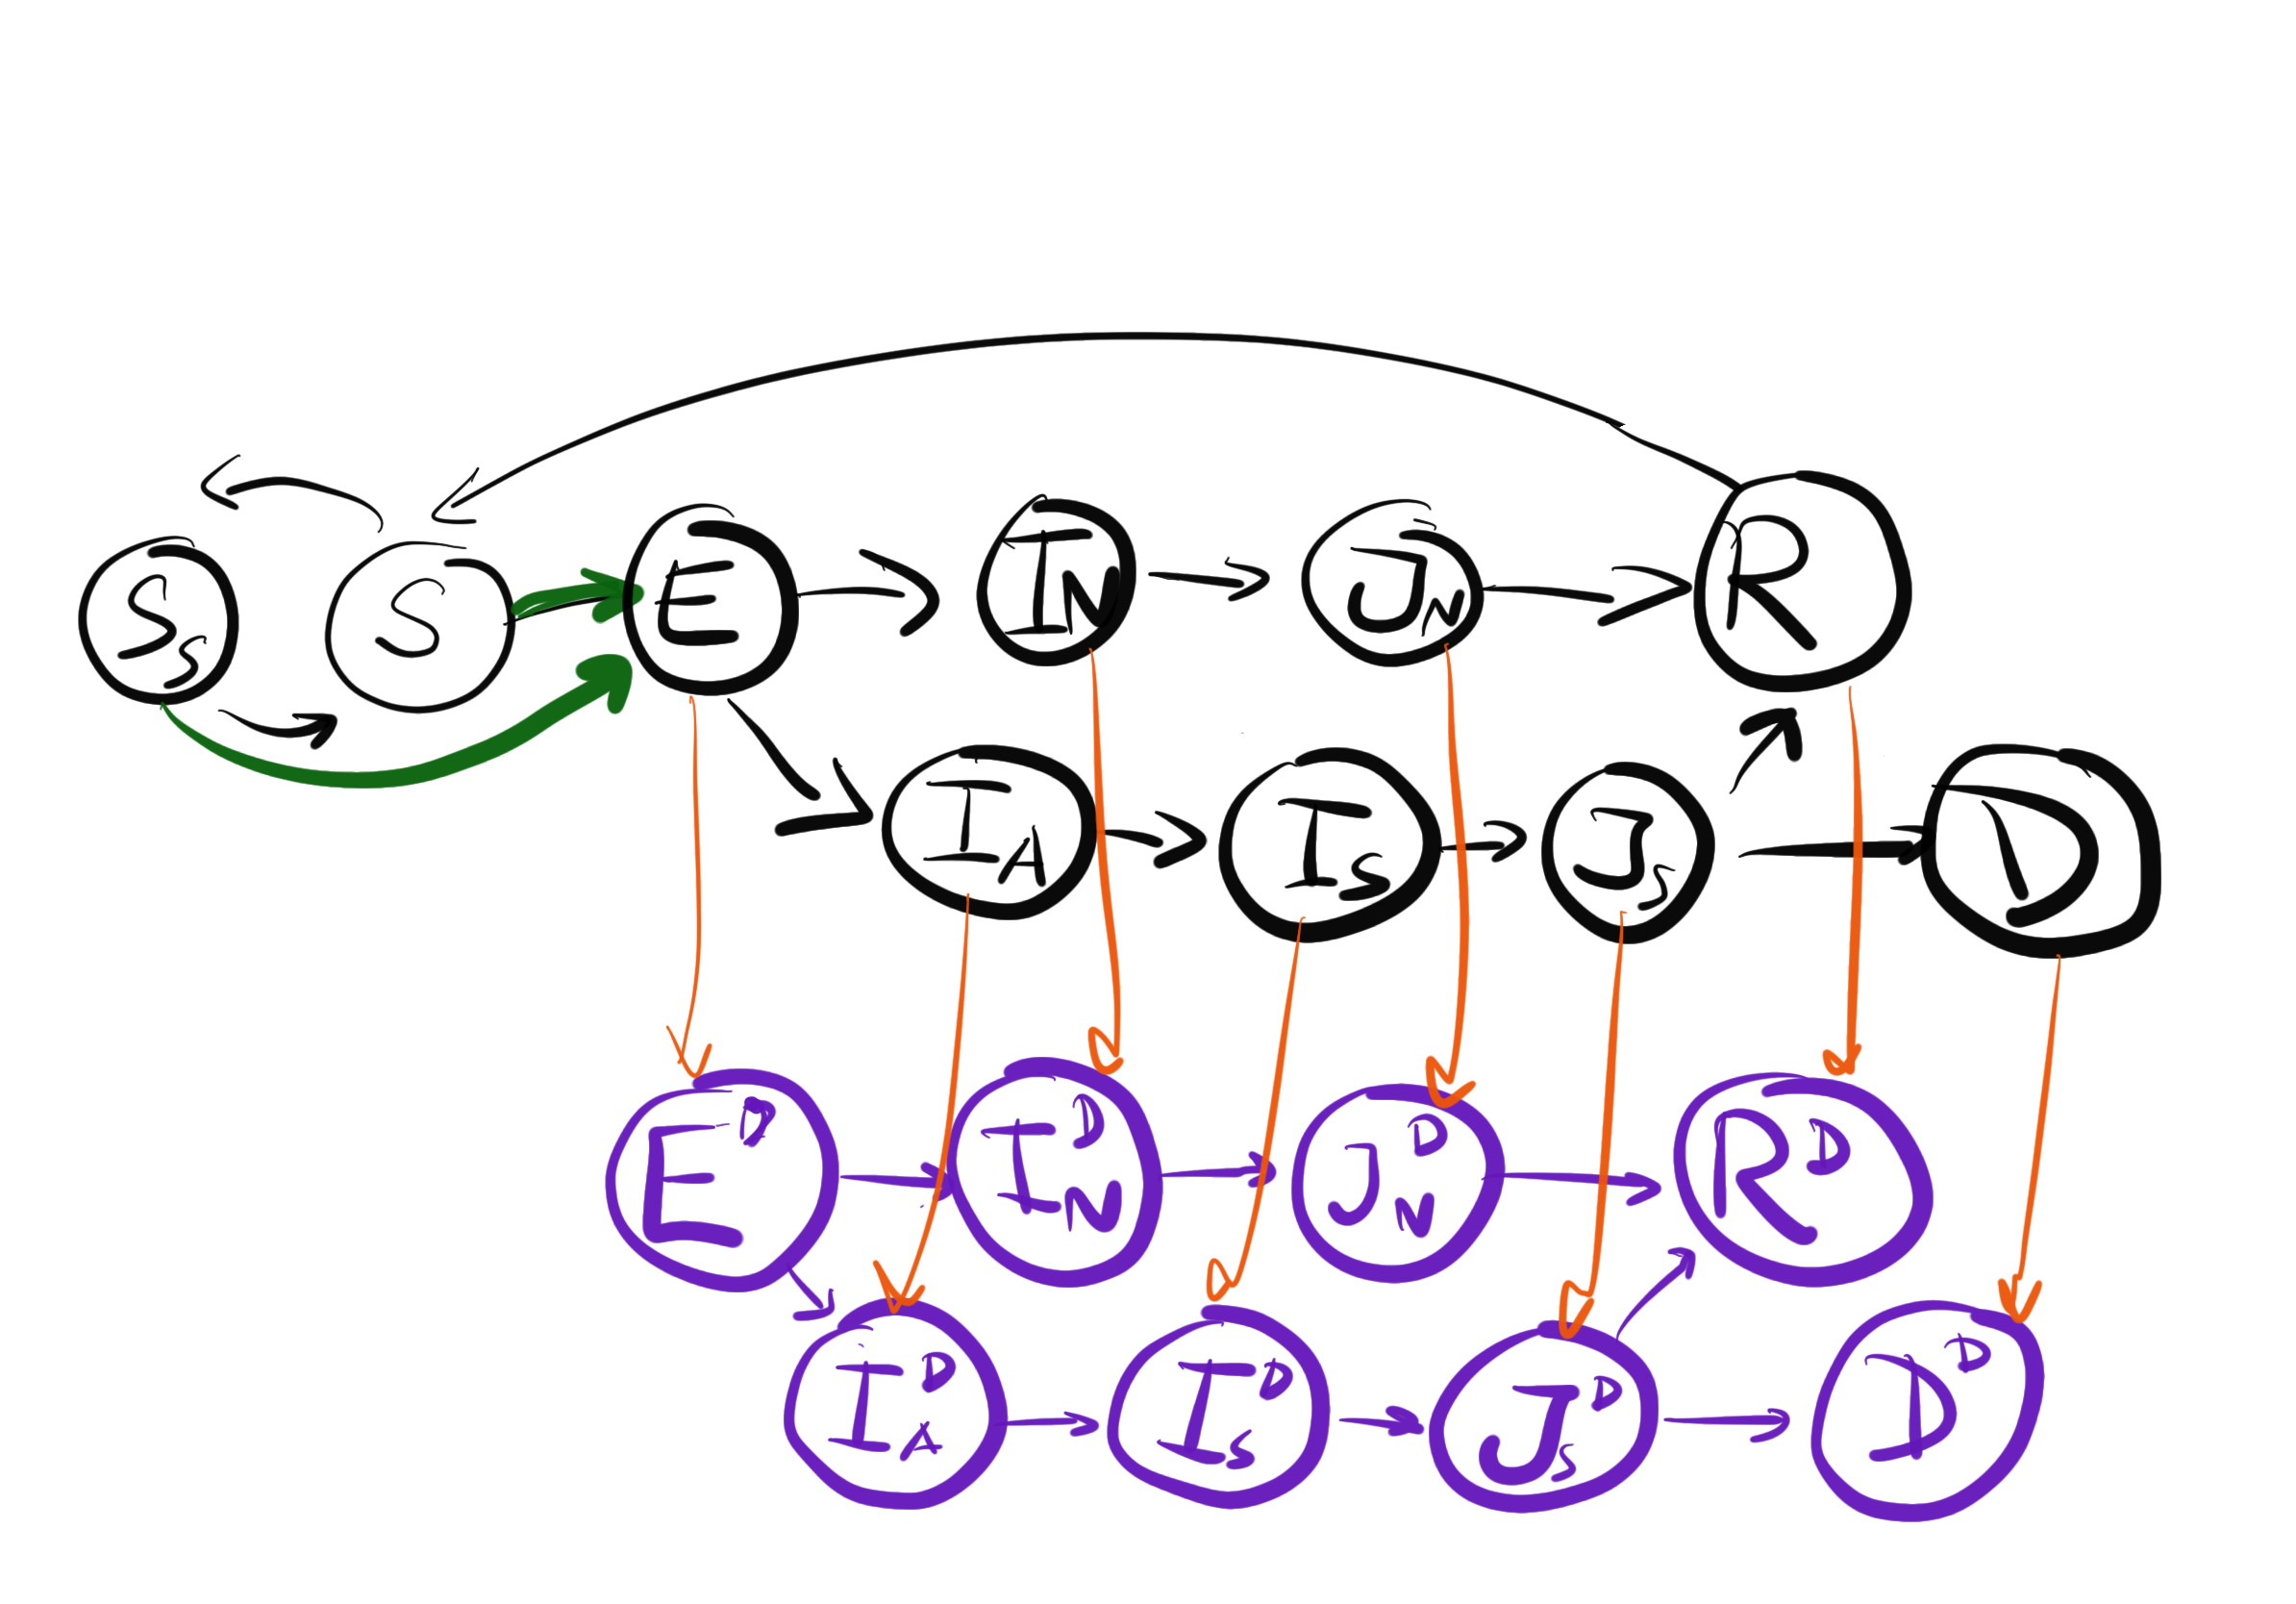
\includegraphics[width=0.99\columnwidth]{pic/epi08}%
}
\caption{Model stavů agenta. Popis stavů je uveden v~Tab.~\ref{tab:states}. Šipky znázoňují možné přechody mezi stavy. Zelené šipky označují nakažení, oranžové šipky jsou přechody způsobené testováním.}%
\label{fig:model-states}%
\end{figure}


\begin{table}
\centering
  \begin{tabular}{lp{.8\textwidth}}
    \hline
		Stav & popis \\\hline
    {\bf $S$} & náchylný k~infekci (susceptible)\\
    {\bf $S_{\bf s}$} & falešně symptomatický (má příznaky ale není nakažen COVID-19)\\ 
    {\bf $E$, $E^d$} & infikovaný v~latentní inkubační fázi, ještě není infekční (exposed) \\
    {\bf $I_{a}$, $I^d_{a}$} & infekční presymptomatický (později bude mít příznaky) \\
    {\bf $I_{s}$, $I^d_{s}$} & infekční symptomatický \\ 
    {\bf $J_{s}$, $J^d_{s}$} & (již) neinfekční symptomatický \\ 
    {\bf $I_{n}$, $I^d_{n}$} & infekční asymptomatický (nikdy nebude mít příznaky) \\ 
    {\bf $J_{ n}$, $J^d_{n}$} & neinfekční asymptomatický \\ 
    {\bf $R$, $R^{d}$} & vyléčený \\
    {\bf $D$, $D^{d}$} & mrtvý  \\
    \hline
  \end{tabular}
  \caption{Seznam stavů agenta. Horní index $d$ označuje stavy agenta, který byl otestován a detekován. Dolní index $s$ označuje symptomy a dolní index $n$ asymptomatický průběh. Typická posloupnost přechodů mezi stavy je $ S \rightarrow  E \rightarrow I_n \rightarrow J_n \rightarrow R$ při asymptomatickém průběh nemoci a $S \rightarrow E \rightarrow I_a \rightarrow I_s \rightarrow J_s \rightarrow R/D$ pro agenty, kteří mají průběh se symptomy.}
  \label{tab:states}
\end{table} 

Přechody mezi stavy jsou realizovány pravděpodobnostně a závisí na vlastnostech nemoci COVID-19. V~tabulce~\ref{paramtab} uvádíme hlavní epidemiologické parametry modelu, které ovlivňují přechody mezi jednotlivými stavy. V~modelu máme několik typů přechodů. Všude tam, kde je možno z~jednoho stavu přejít do více stavů, musíme určit jejich pravděpodobnosti přechodu. To se týká například rozhodování o~symptomatickém nebo asymptomatickém průběhu nemoci, stavu s~falešnými symptomy, nebo úmrtí. 

Další typ přechodu je charakterizován časem, který agent v~daném stavu stráví. Víme například, že průměrná doba inkubace je 5 dní. V~tradičních SEIR modelech simulujeme tento přechod pomocí konstantní pravděpodobnosti přechodu, na jejímž základě každý den přesuneme část populace mezi stavy.\footnote{Zde konkrétně ze stavu $E$ do jednoho ze stavů $I_a$ nebo $I_n$, který z~nich to bude nám určí pravděpodobnost $p_n$ z~tabulky~\ref{paramtab}.} Tento typ přechodu se nazývá Markovovský a odpovídá exponenciálnímu rozdělení setrvání v~daném stavu. Jeho vlastností je, že pravděpodobnost přechodu je každý den stejná, což je ale velké zjednodušení. Podrobnější data a průběhu nemoci nám ukazují, že pravděpodobnosti přechodů mezi stavy se výrazně liší v~závislosti na dnech strávených v~daném stavu. Agentní simulace nám jednoduše umožní generovat doby strávené v~jednotlivých stavech ne-Markovovsky na základě rozdělení pravděpodobnosti odpovídající realitě. Obrázek~\ref{fig:times-states} ukazuje několik takových rozdělení, která jsme modelovali na základě empirických dat z~prací uvedených v~tabulce~\ref{paramtab}.   


\begin{table}
\begin{threeparttable}
\begin{center}
\footnotesize
\begin{tabular}{rp{2.5cm}rp{2.4cm}l}
\hline
Par.&	popis &	hodnota &	chyba &	zdroj \\ \hline\hline
$m_E$&	 doba inkubačního stavu $E$ 	&$5.08$&	95\%CI 4.77-5.39, SD 0.18&	\cite{he2020estimation}	\\
$m_i$&	 doba infekčního stavu  	&$4.76$& 95\%CI 3.44--5.11	&	ECDC\tnote{*}	\\
$m_a$&	 doba presymptomatického stavu 	&$4$&	IQR2-7&	\cite{nie2020epidemiological}	\\
$m_s$&	 doba RNA pozitivity pro symptomatické 	&$25.2$&	SD 4.9&	\cite{noh2020asymptomatic}	\\
$m_n$&	 doba RNA pozitivity pro asymptomatické 	&$22.6$&	SD 4.0&	\cite{noh2020asymptomatic}	\\
$p_n$&	 pravděpodobnost asymptomatického průběhu 	&$0.179$&	95\%CI 15.5--20.2&	\cite{Mizumoto:2020}	\\
$c$&	 míra smrtnosti 	&$0.018$&	95\%CI 0.0118-0.0243, SD 0.0032&	\cite{he2020estimation}	\\
$f$&	 míra falešných příznaků 	&$0.0003$&	&	\cite{szu2020}	\\
$m_f$&	 doba trvání falešných příznaků 	&$5.5$&	&	\cite{szu2020}	\\
\hline
\end{tabular}
\begin{tablenotes}
\item [*] {Údaj z webu ECDC \url{https://www.ecdc.europa.eu/en/covid-19/latest-evidence/infection} pro hodnotu \emph{viral shedding}, detekovatelnosti viru testem PCR z respiračních vzorků. Některé rané práce, jako např.~\cite{wolfel2020virological} uvádějí při datech hospitalizovaných pacientů vyšší střední hodnoty.}
\end{tablenotes}
\caption{Hlavní epidemiologické parametry modelu s~uvedením bibliografického zdroje. Doby trvání jsou vyjádřeny ve dnech, míry a pravděpodobnosti jsou hodnoty z~intervalu $\langle 0,1 \rangle$. }
\label{paramtab}
\end{center}
\end{threeparttable}
\end{table}

\begin{figure}%
\centerline{%
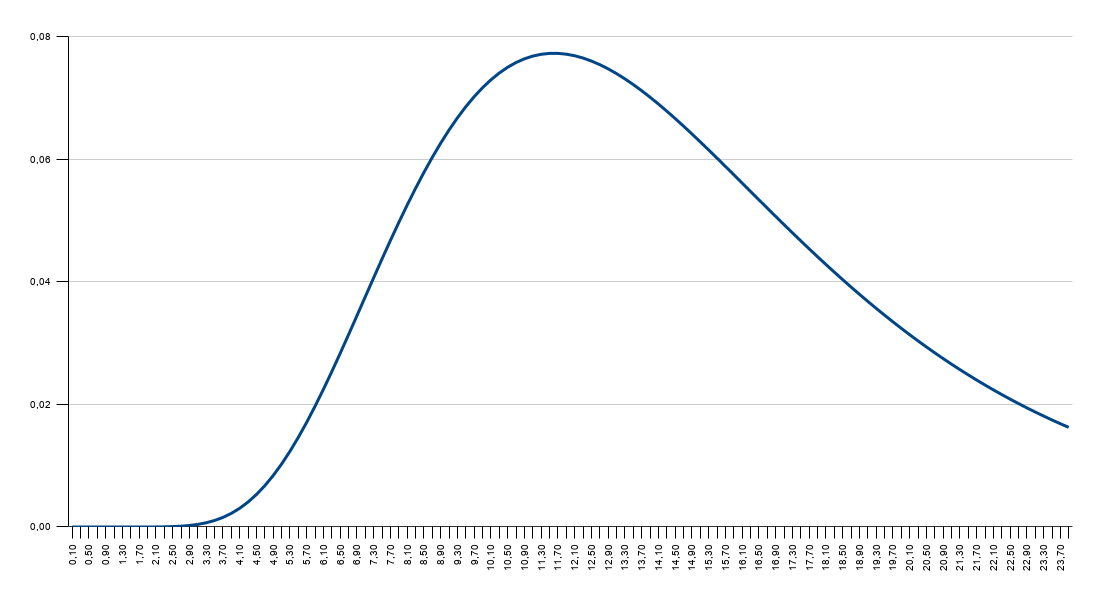
\includegraphics[width=0.49\columnwidth]{pic/time-rna}%
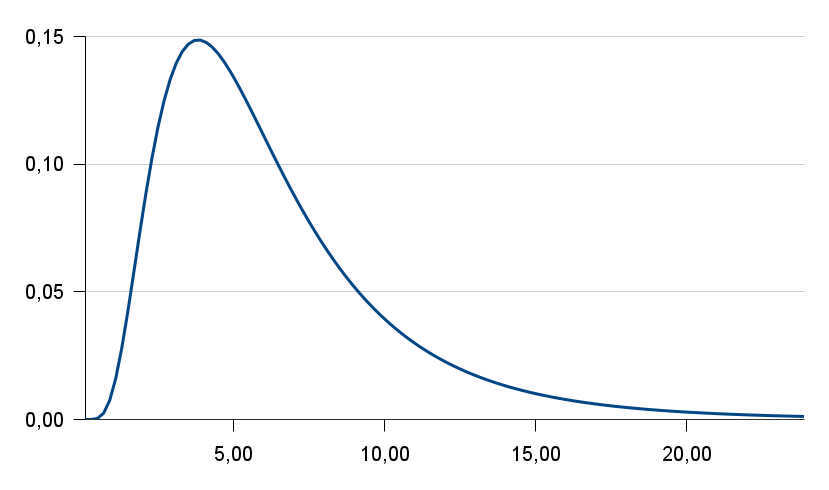
\includegraphics[width=0.49\columnwidth]{pic/time-ink}}
\centerline{%
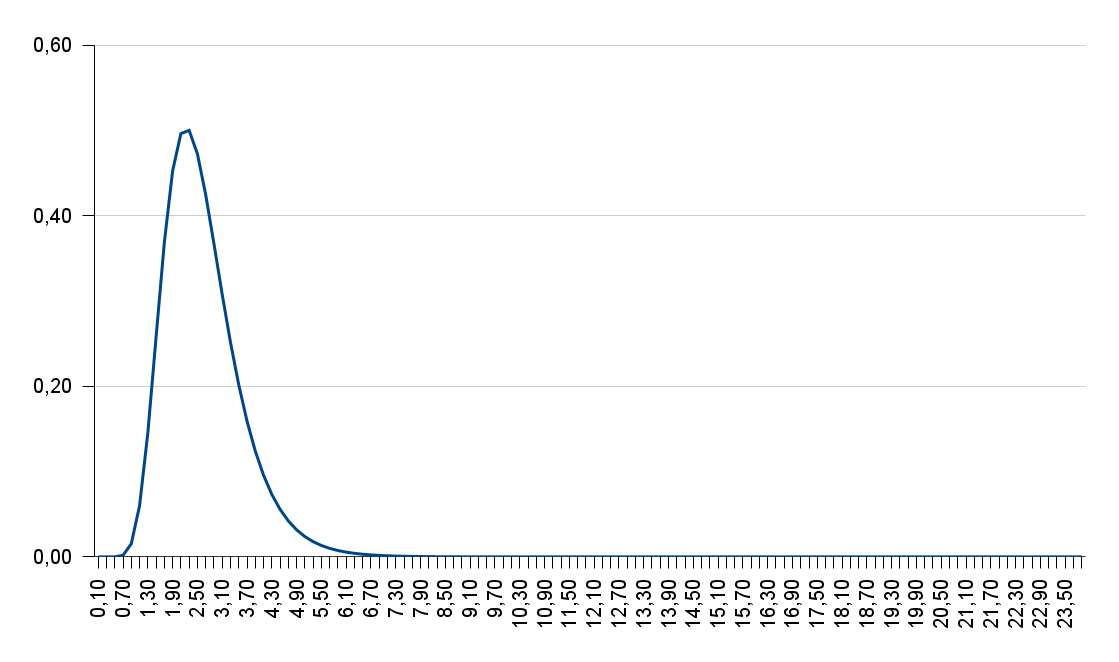
\includegraphics[width=0.49\columnwidth]{pic/time-pre}%
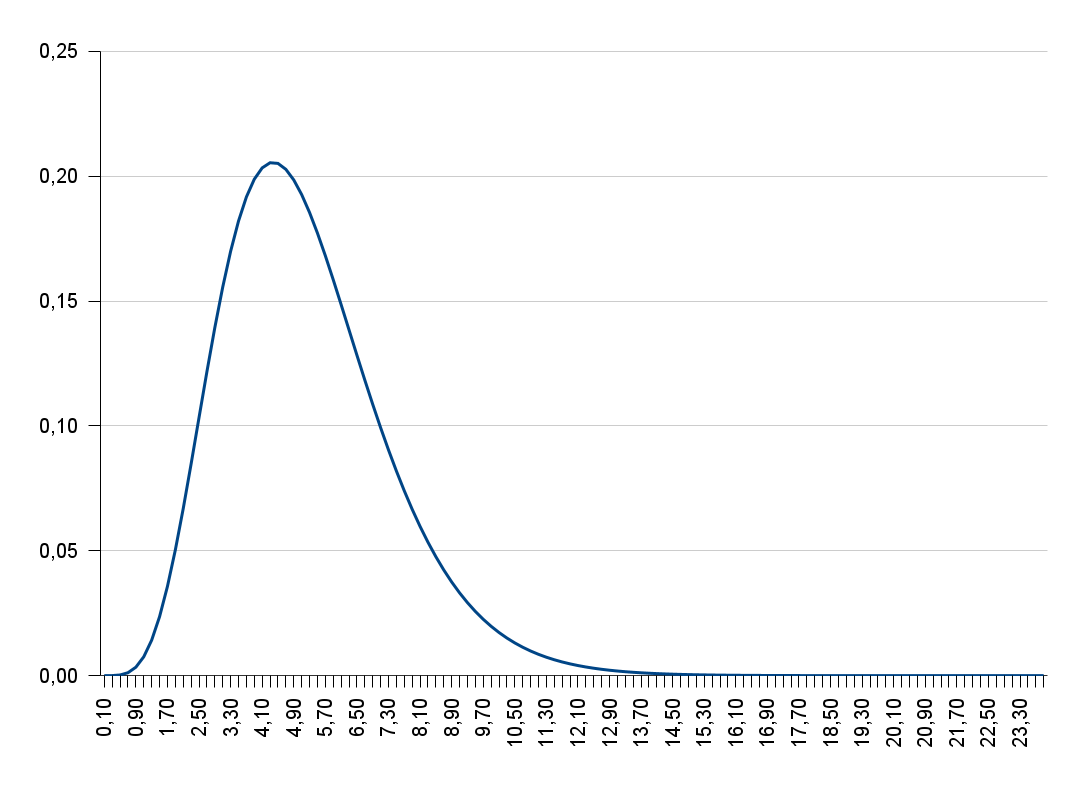
\includegraphics[width=0.49\columnwidth]{pic/time-inf}%
}
\caption{Rozdělení pravděpodobností pro čas strávený v~epidemiologicky významných stavech -- RNA pozitivita (nahoře vlevo), inkubační doba (nahoře vpravo), presymptomatičnost (dole vlevo), infekčnost (dole vpravo). Na ose x jsou dny, na ose y pravděpodobnost že doba trvání stavu bude daný počet dní. Křivky tak znázorňují aproximaci hustoty rozdělení pravděpodobností pro dobu strávenou v~daném stavu.}%
\label{fig:times-states}%
\end{figure}

Nejsložitější typ přechodu představuje vlastní nakažení, tedy přechod $S\to E$. Při tomto přechodu je třeba uvažovat kontakty jedince, identifikovat mezi nimi ty, kteří jsou nakažliví, a na základě vlastností kontaktu (jak dlouho trval, jak byl intenzivní, jaká byla individuální ochranná opatření) a parametru nakažlivosti nemoci, určit, zda k~nakažení dojde. K~dobrému modelování tohoto přechodu se využívá sociální síť kontaktů, o~které si řekneme dále. 

Mnoho parametrů, o~kterých jsme hovořili, můžeme pro jednotlivé agenty nastavit individuálně. Při generování věrné syntetické populace, známe o~každém jedinci řadu detailů, například věk nebo pohlaví, takže parametry související s~nemocí nebo sociální aktivitou lze snadno přizpůsobit. 




\subsubsection*{Kontakty a opatření}

Graf kontaktů agentů definuje prostředí multi-agentního systému, v~rámci kterého spolu agenti interagují. V~předchozí části jsme ukázali, že kontakty hrají klíčovou roli při simulaci nakažení jedince. Zatímco modely založené na rovnicích pracují s~homogenním modelem populace, dobrý graf kontaktů nám u~agentního modelu umožní zohlednit heterogenitu v~počtu i typu kontaktů. Teoretický výzkum v~sociálních vědách i příklady z~reálného šíření epidemie ukazují, že heterogenní rozložení kontaktů je klíčové. Ohniska epidemie často vznikají na základě  událostí, kde dojde ke kumulaci lidí a nakažení velkého počtu lidí. Lidé s~velkým počtem kontaktů mohou působit jako super-přenašeči zodpovědní za stovky nakažených.  

V~našem modelu je vytvoření realistické a podrobné sítě kontaktů klíčové, proto jsme koncept grafu s~agenty jako uzly a kontakty reprezentované hranami zobecnili ve dvou oblastech. První je rozlišení různých typů kontaktů, což vede k~definici sítě kontaktů jako multi-grafu, kde mezi uzly může být více kontaktů (hran) různého typu. Lidé ve městě se potkávají v~rodině, v~práci, při nakupování, atd. To vede k~definování vrstev v~grafu podle typů kontaktů. Vrstva odpovídá kontaktům jednoho typu a má tedy některé společné parametry související s~délkou a intenzitou kontaktu. Druhým zobecněním je zavedení váhy hrany v~grafu, která postihne individuální rozdíly v~kontaktech. Například v~rámci vrstvy kontaktů žáků jedné třídy ve škole můžeme rozlišit žáky, kteří spolu sedí v~lavici. 

Podrobný multi-graf kontaktů umožní i modelování různých protiepidemických opatření. K~nejčastějším nefarmaceutickým opatřením patří globální uzávěry, které se dají velmi snadno implementovat pomocí vrstev v~grafu. Uzavření obchodů nebo restaurací se například snadno modeluje vypnutím odpovídající vrstvy kontaktů. Stejně tak omezení mobility lidí získané na základě sociologických výzkumů dokážeme snadno simulovat vážením dané vrstvy kontaktů relativní četností kontaktů.

Při modelování efektivity dohledávání kontaktů nakažených lidí hrají vrstvy také důležitou úlohu. Míra toho, jaké kontakty nahlásí spolupracující nakažený výrazně závisí na typu kontaktu. Rodinné příslušníky nebo kolegy z~práce, které jsme nedávno potkali, si vybavíme asi všechny, ale kontakty z~návštěvy restaurace budou méně spolehlivé, a kontakty z~obchodů či dopravních prostředků dokážeme dohledat leda použitím technologií jako je trasování pomocí mobilních aplikací.

V~následujících dvou sekcích si stručně ukážeme, jak vypadá modelování epidemie a odpovídajících protiepidemických opatření ve dvou konkrétních prostředích. 

%\subsubsection*{Opatření a dynamika}


%\subsection*{Verona}

\subsection*{Okres na východě}

První případovou studií použití našeho modelu s~agenty je srovnání protiepidemických opatření na základě podrobného modelu okresu Hodonín. Populace Hodonínska se skládá z~56 tisíc obyvatel, z~nichž 24 tisíc žije v~okresním městě a zbytek v~přilehlých obcích. Při generování syntetické populace jsme vycházeli z~dat z~katastru nemovitostí a údajích o~rozmístění škol, firem, obchodů, restaurací, linek místní hromadné dopravy atd. Multi-graf kontaktů tvoří téměř tři miliony hran ve třiceti vrstvách odpovídajících různým typům kontaktů. Základní statistické rozložení kontaktů vzhledem k~věku jsme odvodili z~výzkumu~\cite{Prem_etal2017}. Intenzity nakažlivosti jednotlivých prostředí jsou založeny na dotazníkovém šetření mezi experty a jeho statistickém vyhodnocení. 

Na tomto modelu lze studovat efektivitu různých globálních opatření a vytvářet scénáře odpovídající skutečnému průběhu epidemie, případně testovat hypotetický alternativní vývoj. Pro simulaci reálných opatření jsme vyvinuli algoritmické procedury testování a trasování, u~kterých lze pomocí parametrů měnit jejich efektivitu, a to jak celkově, tak v~různých vrstvách kontaktů. Opatření typu lockdownu a částečných uzávěr oblastí jako restaurace nebo školy lze také modelovat snadno pomocí vrstev odpovídajících kontaktů. Jemnější scénáře související s~omezením kontaktů lidí v~různých vrstvách vyžadují vytvoření kalendáře změn četností kontaktů, k~čemuž používáme výsledky sociologických šetření~\cite{paqcovid}.   

Výsledky studie jsme publikovali v~\cite{M-techrep2021}. Některé výsledky jsou spíše potvrzením zkušeností z~průběhu epidemie v~České republice. Simulace potvrzují, že pro zvládnutí epidemie je důležitá kombinace omezení kontaktů, typicky iniciovaná globálními opatřeními, a individuálních ochranných opatření jako je nošení respirátorů. Další výsledky ukazují důležitost efektivních procedur testování a trasování kontaktů. Je zajímavé, že ideální trasování pomocí elektronických zařízení není tak významné, kromě událostí typu velkých shromáždění lidí v~době, kdy neexistují další omezení kontaktů, tam je naopak dohledání všech kontaktů klíčové k~prevenci vzniku lokálních ohnisek nákazy. Další poznatky o~tomto modelu přinášejí kapitoly~\ref{Grafy_kontaktu}
a~\ref{Evaluace_politik}.


\subsection*{Škola v~centru}

Základní agentní model s~jinou sítí kontaktů a jinými algoritmy protiepidemických opatření byl použit pro modelování bezpečného provozu škol. Řada parametrů souvisejících s~nemocí COVID-19 a relativní nakažlivostí prostředí byla převzata z~před\-cho\-zí studie. Síť kontaktů vznikla na základě specializované dotazníkové studie na pražské základní škole. Syntetická populace agentů v~tomto případě obsahuje 624 žáků a 55 učitelů. Jejich kontakty představují multi-graf s~28 tisíci hran v~98 vrstvách, které zachycují jednotlivé třídy, kontakty na chodbách, v~jídelně, v~kabinetech apod. 

Algoritmy protiepidemických opatření v~prostředí školy odrážejí reálně uvažovaná opatření omezení výuky. Jedná se hlavně o~varianty střídavé docházky, rozdělení školy na stupně, případně kritické ročníky (první, druhý a devátý). Dalším typem opatření jsou různé strategie testování s~ohledem na jejich četnost i efektivitu (antigenní a PCR testy.)

Výsledky studie ukazují efektivitu týdenních rotací celých tříd, která se ještě zesiluje pravidelným testováním. Efektivita testů je v~tomto případě méně důležitá a lze ji nahradit vyšší frekvencí testování. Podrobnější výsledky této studie popisuje kapitola~\ref{Skoly}.

%\cite{model-M}






\section*{Diskuse} 

V~tomto příspěvku jsme ukázali princip vytváření agentních síťových epidemiologických modelů, které umožňují detailní pohled na šíření epidemie na úrovní jedinců. Tyto modely jsou flexibilní a dokáží popsat dynamiku  epidemie v~různých prostředích, jako je město nebo škola. Algoritmické procedury simulace epidemiologických opatření slouží k~porovnání efektivity lokálních uzávěr, testování a trasování, nebo vakcinačních strategií. 

S~úrovní detailů agentních modelů na realistických sítích kontaktů souvisí i jejich nevýhody. Model má mnohem více parametrů než kompartmentové protějšky, hodnoty těchto parametrů je třeba pečlivě nastavit případně doladit pomocí optimalizačních procedur. Stochastické simulace průběhu epidemie zase vyžadují provést velké množství spuštění modelu a jejich statistické vyhodnocení, protože výsledky mohou mít velký rozptyl. Modely s~agenty jsou tak vhodnější pro relativní srovnání různých scénářů než k~absolutní předpovědi průběhu epidemie. 

Snažili jsme se modely s~agenty představit v~kontextu teoretických věd, jako je informatika a teorie grafů, i jejich praktických aplikací v~přírodních a společenských vědách. Vývoj v~jednotlivých disciplínách probíhá často odděleně a jednotlivé proudy spolu nekomunikují. Z~našich zkušeností ale vyplývá, že tvorba agentního epidemiologického modelu je multidisciplinární a neobejde se bez spolupráce informatiků, statistiků, epidemiologů, sociologů a dalších odborníků.\footnote{Popsaný model je k~dispozici jako volný software na adrese \url{https://github.com/epicity-cz/model-m/releases/tag/v0.3}} 
